\setRL
%\pagenumbering{arabic} 


\section{\label{sec:nuclearenvelope}
بسته‌ی هسته‌ی سلول
}
غشای هسته یا نام رایج آن، بسته‌ی هسته
\LTRfootnote{nuclear envelope}
ساختاری متفاوت نسبت به غشای سلول دارد. در خارج و اطراف هسته، ساختارهای زیادی وجود دارد، مانند شبکه‌ی اکتین
\LTRfootnote{actin network}
 و میکروتیوبول‌ها
\LTRfootnote{microtubules}
. هسته‌ی سلول از طریق بسته‌ی هسته با تمامی‌ ارگان‌های لازم در ارتباط است.

در شکل 
\ref{fig:nuclearenvelope}
نقاشی از ساختار کلی بسته‌ی هسته را می‌بینیم. از بالا به پایین، خطوط زرد رنگ نماینده‌ی شبکه‌ی پروتئینی اکتین است. این شبکه از طریق پروتئین‌هایی به نام نسپرین
\LTRfootnote{nesprin}
، که روی بسته‌ی هسته وجود دارند، به بسته‌ی هسته متصل است و نقش پلی برای انتقال نیرو‌های خارج از سلول به هسته‌ی سلول را ایفا می‌کند
\cite{Lammerding2011}. بسته‌ی هسته از ۲ عدد غشای لیپیدی دو لایه (نوارهای صورتی) با نام غشای بیرونی و غشای داخلی تشکیل شده. ضخامت فضای بین دو غشا از ۲۰ تا ۴۰ نانومتر تغییر می‌کند. میان دو غشا را مایعی شبیه به سیتوپلاسم و شبکه‌ای پروتئینی، لازم برای انتقال مواد بین هسته و سلول، پر می‌کند. پروتئین‌های نسپرین  در غشای داخلی هم حضور دارد و این غشا را به شبکه‌ی پروتئینی لمینا
\LTRfootnote{lamina}
(شکل
\ref{fig:nuclearenvelope}
نقاشی سمت چپ، خطوط سبز‌ رنگ) متصل می‌کند. لمینا‌ شبکه‌ای است به ضخامت حدود ۵۰ تا ۸۰ نانومتر که تمام سطح غشای داخلی را پوشانده است. در تصویر سمت راست شکل 
\ref{fig:nuclearenvelope}
با استفاده از روش‌های رنگامیزی میکروسکوپی، لایه‌ی لمینا را به رنگ سبز روشن می‌بینیم که کروماتین‌های (قرمز) درون هسته را محصور کرده‌اند. لمینا خاصیت الاستیکی دارد و تقریبا تمام ویژگی الاستیک بسته‌ی هسته به علت وجود این بخش است
\cite{Steensel2017wd}
. 


\begin{figure}[h]
\begin{center}
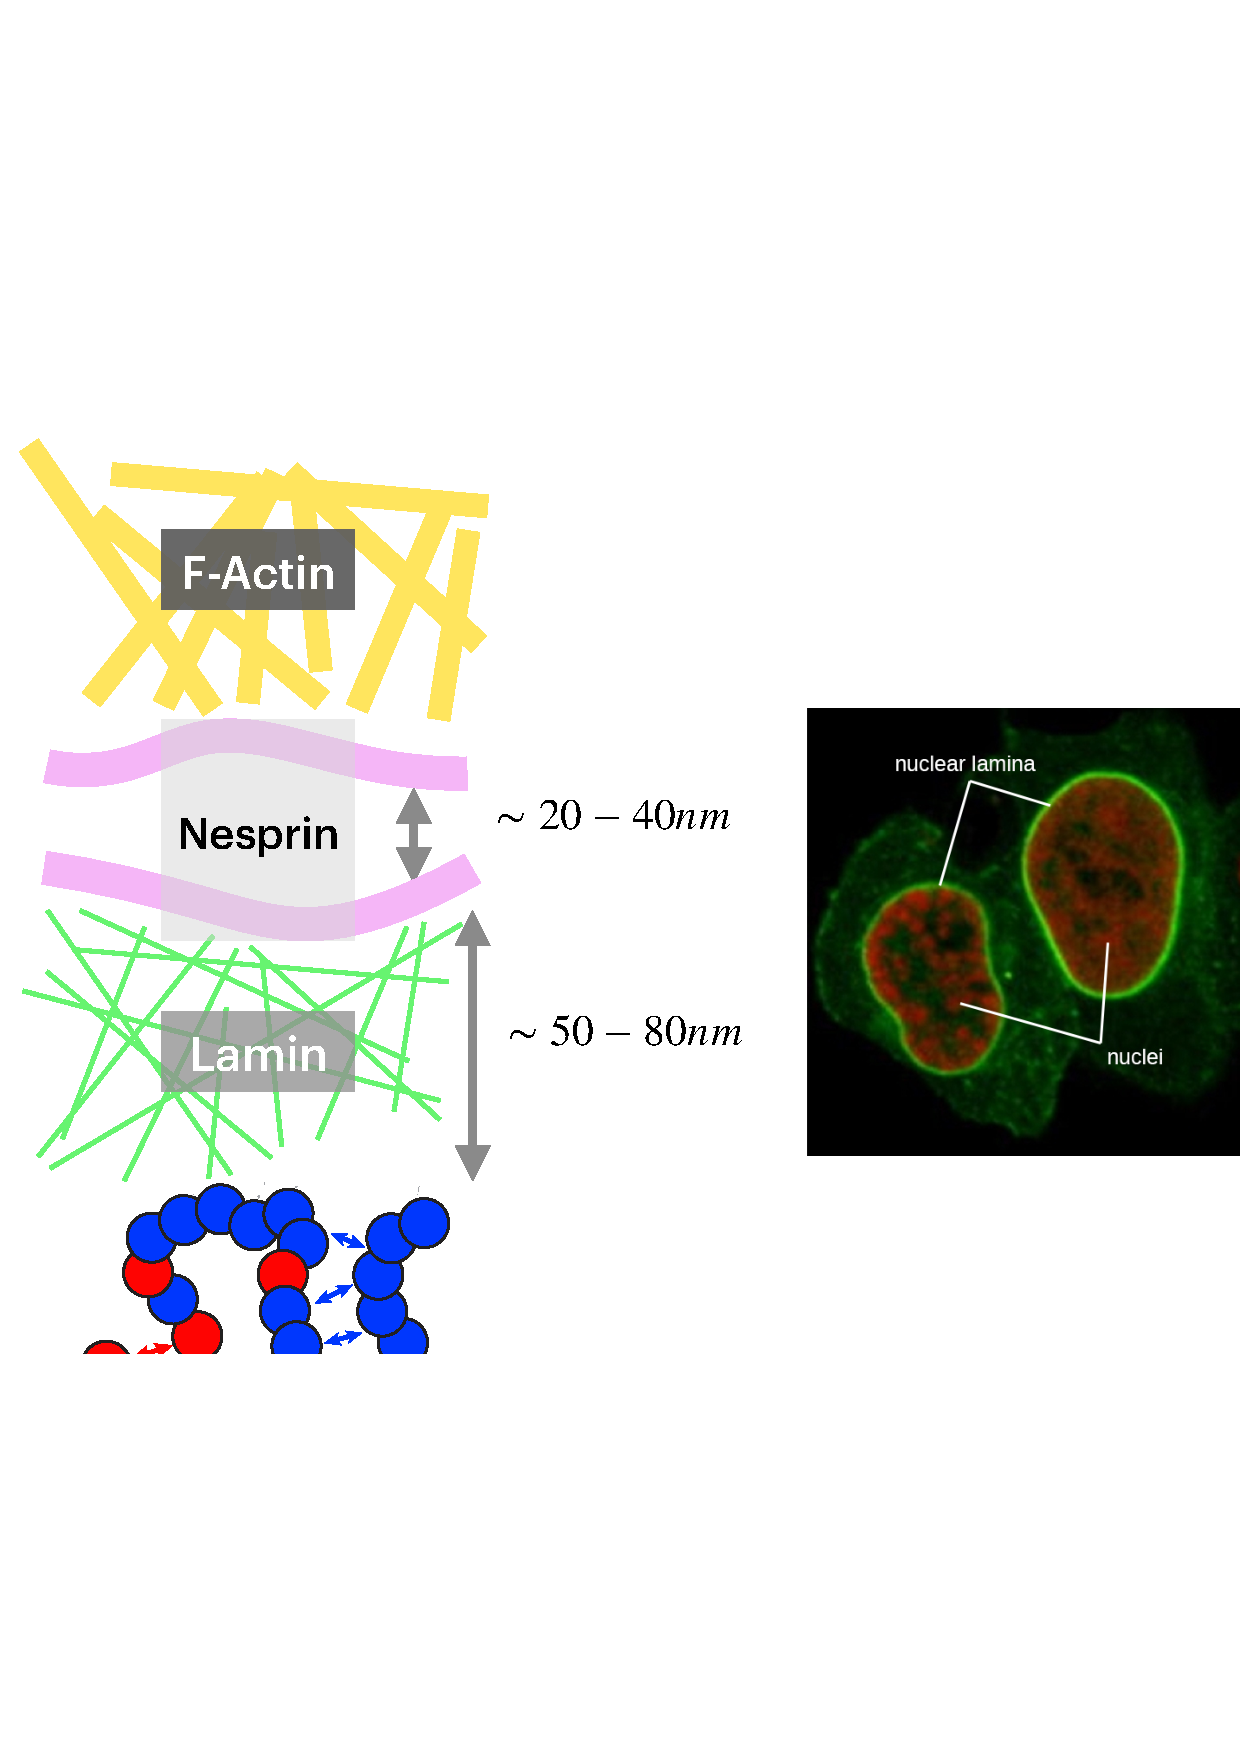
\includegraphics[width=3.5in]{\MemBio /Pics/NuclearEnvelope}
\caption{
عکس سمت راست، تصویر رنگامیزی شده‌ی هسته. لایه‌ی لمینا با رنگ سبز روشن، و کروماتین‌های درون هسته با رنگ قرمز نمایش داده‌ شده‌است. شکل سمت چپ، نقاشی ساختار بسته‌ی هسته است. از بالا به پایین: شبکه‌ی اکتین (زرد) که با پروتئین‌های نسپرین به غشای دولایه‌ی بیرونی (نوار صورتی) متصل شده‌است. غشای داخلی نیز به کمک همین پروتئین به لایه‌ی لمینا (سبز) متصل شده. فضای میان غشای داخلی و خارجی از ۲۰ تا ۴۰ نانومتر تغییر می‌کند. ضخامت لمینا نیز بین ۵۰ تا ۸۰ نانومتر است. کروماتین‌های درون هسته نیز (دایره‌های آبی و قرمز) با لایه‌ی لمینا اتصالاتی برقرار می‌کند. 
}
\label{fig:nuclearenvelope}
\end{center}
\end{figure}
مدول الاستیک شبکه‌ی اکتین تقریبا ۵۰۰ پاسکال، و مدول الاستیک هسته‌ی سلول زمانی که درون سلول قرار دارد، ۵ هزار پاسکال و هنگامی ‌که از سلول خارج شده باشد، ۸ هزار پاسکال اندازه‌گیری شده‌است
\cite{Dahl2004, CAILLE2002177}.







